\documentclass[border=0.1cm]{standalone}
\usepackage{tikz}

\begin{document}


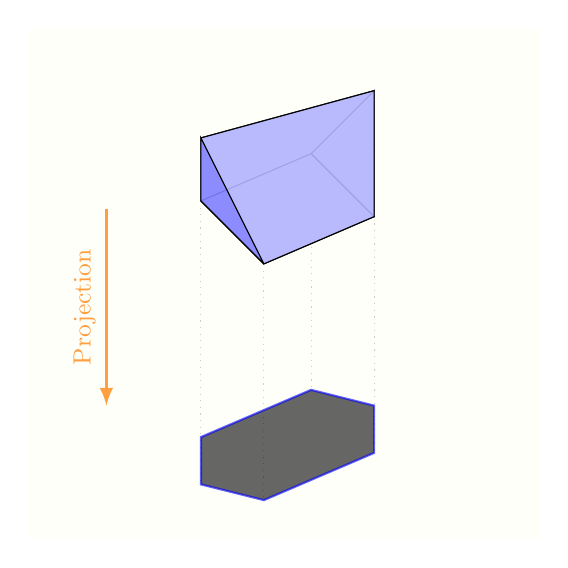
\begin{tikzpicture}
\fill[yellow!2] (-3,-3.5) rectangle (3.5,3);
\begin{scope}
\draw[dotted,black!20] (0,0) -- (0,-3)(1.4,0.6)--(1.4,-2.4)(0.6,1.4) -- (0.6,-1.6)(-0.8,0.8) -- (-0.8,-2.8)(1.4,2.2) -- (1.4,-1.8)(-0.8,1.6)(-0.8,-2.2);
\draw[draw=blue,thick,fill=black,opacity=0.6,yshift=-0.5cm] (0,-2.5) -- (1.4,-1.9) -- (1.4,-1.3) -- (0.6,-1.1) -- (-0.8,-1.7) -- (-0.8,-2.3) -- cycle;
\end{scope}
\draw[very thick,-latex,orange!75] (-2,0.7) -- (-2,-1.8) node[sloped,midway,above,rotate=180]{\small Projection};

\draw (0,0) -- (1.4,0.6) -- (0.6,1.4) -- (-0.8,0.8) -- cycle;
\draw (1.4,0.6) -- (1.4,2.2) --(0.6,1.4); 


\draw (0,0) -- (-0.8,1.6) -- (-0.8,0.8)(-0.8,1.6) --(1.4,2.2) ;

\fill[blue!30,opacity=0.9] (-0.8,1.6)--(1.4,2.2) --(1.4,0.6) -- (0,0) -- cycle;
\fill[blue!50,opacity=0.9] (-0.8,1.6)--(-0.8,0.8) --(0,0);

\draw (0,0) -- (-0.8,1.6) -- (-0.8,0.8) -- (0,0) --(1.4,0.6) -- (1.4,2.2) --(-0.8,1.6) ;




%\draw[yshift=-2.5cm] (-2,-0.4285*2) -- (2,0.4285*2);
%\draw[yshift=-1.35cm] (-2,-0.4285*2) -- (2,0.4285*2);

%\draw[step=1,lightgray,rotate=23.2,transform canvas={yshift=0.35cm}] (-4,-6) grid (2,-1);

%\draw (1.4,-1.3) -- (-0.8,-2.3);

\end{tikzpicture}


\end{document}
